
\documentclass[11pt,a4paper]{article}

% ---------- Ngôn ngữ & phông chữ (XeLaTeX + Liberation Serif) ----------
\usepackage{fontspec}
\usepackage{polyglossia}
\setdefaultlanguage{vietnamese}
\setmainfont{Liberation Serif}
\setsansfont{Liberation Sans}
\setmonofont{Liberation Mono}[Scale=0.88]

% Ghi chú: KHÔNG dùng unicode-math ở đây. Gói đó ánh xạ lại họ font toán,
% làm hỏng ký tự dấu ngoặc mở rộng của \underbrace (amsmath). Bộ toán cổ
% điển Latin Modern dưới đây tương thích hoàn toàn với XeLaTeX.

% ---------- Trình bày trang ----------
\usepackage[a4paper,margin=2.6cm]{geometry}
\usepackage{microtype}
\usepackage{fancyhdr}
\usepackage{titlesec}

% ---------- Toán học ----------
\usepackage{amsmath, amssymb, amsthm, mathtools}
\usepackage{bm}

% ---------- Bảng, hình, thuật toán, mã nguồn ----------
\usepackage{booktabs}
\usepackage{graphicx}
\usepackage{caption}
\usepackage{subcaption}
\usepackage{float}
\usepackage{tikz}
\usetikzlibrary{arrows.meta, positioning}
\usepackage[linesnumbered,ruled,vlined]{algorithm2e}
\usepackage{listings}
\usepackage{xcolor}

% ---------- Siêu liên kết ----------
\usepackage[hidelinks,colorlinks=true,linkcolor=linknavy,
            citecolor=linknavy,urlcolor=linknavy]{hyperref}

%=======================================================================
%  Định nghĩa màu, môi trường định lý, kiểu mã nguồn
%=======================================================================
\definecolor{linknavy}{HTML}{1F4E9C}
\definecolor{codebg}{HTML}{F7F7F9}
\definecolor{codekw}{HTML}{1E8449}
\definecolor{codecm}{HTML}{7F8C8D}
\definecolor{tabhl}{HTML}{EAF2FB}

\theoremstyle{plain}
\newtheorem{theorem}{Định lý}[section]
\newtheorem{lemma}[theorem]{Bổ đề}
\newtheorem{proposition}[theorem]{Mệnh đề}
\newtheorem{corollary}[theorem]{Hệ quả}

\theoremstyle{definition}
\newtheorem{definition}[theorem]{Định nghĩa}
\newtheorem{assumption}[theorem]{Giả thiết}

\theoremstyle{remark}
\newtheorem{remark}[theorem]{Nhận xét}

\renewcommand{\proofname}{Chứng minh}

\lstdefinestyle{py}{
  language=Python, basicstyle=\ttfamily\scriptsize,
  keywordstyle=\color{codekw}\bfseries, commentstyle=\color{codecm}\itshape,
  stringstyle=\color{linknavy}, backgroundcolor=\color{codebg},
  numbers=left, numberstyle=\tiny\color{codecm}, numbersep=7pt,
  frame=single, rulecolor=\color{codecm!40}, breaklines=true,
  showstringspaces=false, columns=fullflexible, xleftmargin=16pt,
  literate={ơ}{{\o}}1 {ư}{{u}}1
}

% ---------- Ký hiệu tắt ----------
\newcommand{\R}{\mathbb{R}}
\newcommand{\Hone}{H^{1}}
\newcommand{\Hzero}{H^{1}_{0}}
\newcommand{\Ltwo}{L^{2}}
\newcommand{\Vh}{V_{h}}
\newcommand{\Rh}{\mathcal{R}_{h}}
\newcommand{\dt}{\Delta t}
\newcommand{\norm}[1]{\left\lVert #1 \right\rVert}
\newcommand{\seminorm}[1]{\left\lvert #1 \right\rvert}
\newcommand{\ip}[2]{\left( #1 , #2 \right)}
\newcommand{\Uvec}{\bm{U}}
\newcommand{\lammax}{\lambda_{\max}}

\pagestyle{fancy}
\fancyhf{}
\fancyhead[L]{\small\itshape FEM cho phương trình sóng một chiều}
\fancyhead[R]{\small\thepage}
\renewcommand{\headrulewidth}{0.4pt}

%=======================================================================
\begin{document}

\begin{titlepage}
\centering
\vspace*{1.6cm}

{\large Trường Đại học Khoa học Tự nhiên -- ĐHQG TP.HCM}\\[0.25cm]
{\large Khoa Toán -- Tin học}\\[2.6cm]

{\Large\bfseries Báo cáo môn học}\\[0.5cm]
{\Large Giải tích số cho Phương trình Đạo hàm riêng}\\[1.4cm]

\rule{\linewidth}{0.5pt}\\[0.55cm]
{\huge\bfseries Phương pháp Phần tử Hữu hạn\\[0.28cm]
cho Phương trình Sóng Một chiều}\\[0.45cm]
{\large\itshape Phân tích ổn định sắc nét và kiểm chứng bậc hội tụ}\\[0.5cm]
\rule{\linewidth}{0.5pt}\\[2.2cm]

{\large
\begin{tabular}{r@{\hspace{0.8em}}l}
\textit{Nhóm thực hiện:} & Nông Thanh Toàn \\[0.2cm]
                         & Nguyễn Hoàng Tú \\
\end{tabular}}\\[2.6cm]

{\large Ngày 29 tháng 7 năm 2026}

\vfill
\end{titlepage}

%=======================================================================
\begin{abstract}
\noindent
Báo cáo trình bày đầy đủ việc xây dựng, phân tích và kiểm chứng số phương
pháp phần tử hữu hạn (FEM) với phần tử tuyến tính từng khúc $P_1$ kết hợp sơ
đồ sai phân trung tâm (leapfrog) cho phương trình sóng một chiều với điều
kiện biên Dirichlet thuần nhất. Ngoài phần dẫn xuất mô hình và chứng minh
hội tụ, đóng góp chính của báo cáo là \emph{phân tích ổn định sắc nét}: bằng
cách tính tường minh phổ của cặp ma trận $(S,T)$, chúng tôi chứng minh điều
kiện ổn định cần và đủ của sơ đồ là
\[
  \dt \;<\; \frac{2}{c\sqrt{\lammax(T^{-1}S)}},
\]
từ đó suy ra hai hằng số CFL khác nhau rõ rệt: $\dt < h/(c\sqrt{3})$ đối với
\emph{ma trận khối lượng đầy đủ} và $\dt < h/c$ đối với \emph{ma trận khối
lượng gộp}. Kết quả này giải thích chính xác vì sao ước lượng quen thuộc
$\dt \le h/c$ là \emph{không đủ} khi dùng khối lượng đầy đủ. Thực nghiệm số
xác nhận ngưỡng lý thuyết tới bốn chữ số có nghĩa, đồng thời tái lập đúng
bậc hội tụ $\mathcal{O}(h^{2})$ trong chuẩn $\Ltwo$ và $\mathcal{O}(h)$
trong nửa chuẩn $\Hone$.

\medskip
\noindent\textbf{Từ khóa:} phương trình sóng, phần tử hữu hạn, sai phân trung
tâm, điều kiện CFL, khối lượng gộp, phép chiếu Ritz.
\end{abstract}

\tableofcontents
\clearpage

%=======================================================================
\section{Giới thiệu}
\label{sec:gioithieu}

Phương trình sóng là mô hình cơ bản mô tả sự lan truyền của dao động cơ học,
sóng âm và sóng điện từ. Do nghiệm giải tích chỉ tồn tại trong một số ít
trường hợp đặc biệt, việc xây dựng lược đồ số vừa \emph{chính xác} vừa
\emph{ổn định} có ý nghĩa thực tiễn lớn.

Bài toán được xét trong báo cáo này là bài toán Dirichlet thuần nhất trên
khoảng đơn vị: tìm $u : [0,1] \times [0,T] \to \R$ sao cho
\begin{equation}
\label{eq:strong}
\left\{
\begin{aligned}
 &\frac{\partial^{2}u}{\partial t^{2}}
   - c^{2}\frac{\partial^{2}u}{\partial x^{2}} = 0,
   && (x,t) \in (0,1)\times(0,T), \\[2pt]
 &u(0,t) = u(1,t) = 0, && t \in (0,T), \\[2pt]
 &u(x,0) = u_{0}(x), \quad \frac{\partial u}{\partial t}(x,0) = u_{1}(x),
   && x \in (0,1),
\end{aligned}
\right.
\end{equation}
với vận tốc truyền sóng $c > 0$ cho trước.

\subsection*{Đóng góp của báo cáo}

\begin{enumerate}
  \item Dẫn xuất đầy đủ dạng yếu, hệ bán rời rạc và lược đồ rời rạc hoàn
        chỉnh, kèm thuật toán Thomas độ phức tạp $\mathcal{O}(N)$ cho mỗi
        bước thời gian (Mục~\ref{sec:khonggian} và \ref{sec:thoigian}).
  \item \textbf{Phân tích ổn định sắc nét} (Mục~\ref{sec:ondinh}): tính tường
        minh phổ suy rộng của $(S,T)$ và chứng minh điều kiện ổn định
        \emph{cần và đủ}, thu được hai hằng số CFL riêng biệt cho khối lượng
        đầy đủ và khối lượng gộp. Đây là điểm mà các trình bày sơ lược
        thường chỉ nêu dưới dạng phỏng đoán.
  \item Chứng minh hội tụ chặt chẽ dựa trên \emph{phép chiếu Ritz}
        (Mục~\ref{sec:hoitu}), nhờ đó tránh được số hạng dư không kiểm soát
        được và không cần viện tới bổ đề Aubin--Nitsche.
  \item Kiểm chứng số hệ thống (Mục~\ref{sec:thucnghiem}): xác nhận bậc hội tụ
        theo cả không gian lẫn thời gian, và định vị ngưỡng ổn định thực
        nghiệm trùng khớp với lý thuyết tới bốn chữ số có nghĩa.
\end{enumerate}

Toàn bộ mã nguồn tái lập kết quả được cung cấp ở Phụ lục~\ref{app:code}.

%=======================================================================
\section{Dạng yếu và tính bảo toàn năng lượng}
\label{sec:dangyeu}

\subsection{Không gian hàm}

Với miền $D \subset \R$, chuẩn $\Ltwo(D)$ của hàm $f$ được định nghĩa bởi
\begin{equation}
\label{eq:l2norm}
  \norm{f}_{\Ltwo(D)}^{2} := \int_{D} \lvert f(x) \rvert^{2}\,dx ,
\end{equation}
và $f$ gọi là \emph{bình phương khả tích} nếu
$\norm{f}_{\Ltwo(D)} < \infty$. Theo bất đẳng thức Cauchy--Schwarz, tích của
hai hàm bình phương khả tích là khả tích, điều này bảo đảm mọi tích phân
xuất hiện dưới đây đều tồn tại.

Không gian Sobolev bậc nhất $\Hone(0,1)$ gồm các hàm bình phương khả tích có
đạo hàm suy rộng cấp một cũng bình phương khả tích. Không gian con các hàm
triệt tiêu trên biên được ký hiệu
\[
  \Hzero(0,1) := \bigl\{ v \in \Hone(0,1) : v(0) = v(1) = 0 \bigr\}.
\]

\subsection{Xây dựng dạng yếu}

Nhân \eqref{eq:strong} với hàm thử $v \in \Hzero$ (không phụ thuộc $t$) rồi
lấy tích phân trên $(0,1)$:
\begin{equation}
\label{eq:multiply}
  \int_{0}^{1}
    \left( \frac{\partial^{2}u}{\partial t^{2}}
         - c^{2}\frac{\partial^{2}u}{\partial x^{2}} \right) v \,dx = 0 .
\end{equation}
Áp dụng tích phân từng phần cho số hạng thứ hai và sử dụng $v(0)=v(1)=0$:
\begin{equation}
\label{eq:byparts}
  \int_{0}^{1} \frac{\partial^{2}u}{\partial x^{2}} v \,dx
  = \underbrace{\left[ \frac{\partial u}{\partial x} v \right]_{0}^{1}}
    _{\textstyle = 0 \ \text{do}\ v \in \Hzero}
    - \int_{0}^{1} \frac{\partial u}{\partial x}
                   \frac{\partial v}{\partial x} \,dx .
\end{equation}
Thay vào \eqref{eq:multiply} ta thu được dạng song tuyến tính
\begin{equation}
\label{eq:bilinear}
  a(u,v) := \int_{0}^{1} \frac{\partial^{2}u}{\partial t^{2}} v \,dx
          + c^{2}\int_{0}^{1} \frac{\partial u}{\partial x}
                              \frac{\partial v}{\partial x} \,dx = 0 .
\end{equation}

\begin{definition}[Dạng yếu của phương trình sóng]
\label{def:weak}
Tìm $u$ sao cho $u(\cdot,t) \in \Hzero$ với mọi $t \in (0,T)$ và
\begin{equation}
\label{eq:weak}
  \ip{u_{tt}(\cdot,t)}{v} + c^{2}\ip{u_{x}(\cdot,t)}{v_{x}} = 0
  \qquad \forall\, v \in \Hzero,\ \forall\, t \in (0,T),
\end{equation}
đồng thời thỏa mãn các điều kiện ban đầu trong \eqref{eq:strong}. Ở đây
$\ip{\cdot}{\cdot}$ ký hiệu tích vô hướng trong $\Ltwo(0,1)$.
\end{definition}

\subsection{Bảo toàn năng lượng ở mức liên tục}

Tính chất sau là kim chỉ nam cho toàn bộ phân tích ổn định về sau: lược đồ
số tốt phải mô phỏng được nó.

\begin{proposition}[Bảo toàn năng lượng]
\label{prop:energy}
Nghiệm đủ trơn của \eqref{eq:weak} bảo toàn năng lượng
\begin{equation}
\label{eq:cont-energy}
  E(t) := \norm{u_{t}(\cdot,t)}_{\Ltwo}^{2}
        + c^{2}\norm{u_{x}(\cdot,t)}_{\Ltwo}^{2},
  \qquad E(t) = E(0) \quad \forall t \in [0,T].
\end{equation}
\end{proposition}

\begin{proof}
Chọn hàm thử $v = u_{t}(\cdot,t) \in \Hzero$ trong \eqref{eq:weak}:
\[
  \ip{u_{tt}}{u_{t}} + c^{2}\ip{u_{x}}{u_{xt}} = 0 .
\]
Do $\ip{u_{tt}}{u_{t}} = \tfrac{1}{2}\tfrac{d}{dt}\norm{u_{t}}^{2}$ và
$\ip{u_{x}}{u_{xt}} = \tfrac{1}{2}\tfrac{d}{dt}\norm{u_{x}}^{2}$, ta được
$\tfrac{1}{2}\tfrac{d}{dt}E(t) = 0$, tức $E$ là hằng số.
\end{proof}

%=======================================================================
\section{Rời rạc hóa không gian}
\label{sec:khonggian}

\subsection{Lưới, nút và phần tử}

Chia $[0,1]$ thành $N$ phần tử bằng nhau với kích thước $h = 1/N$. Các nút và
phần tử được định nghĩa bởi
\begin{equation}
\label{eq:mesh}
  x_{i} := (i-1)h,\quad i = 1,\dots,N+1,
  \qquad
  E_{i} := [x_{i}, x_{i+1}],\quad i = 1,\dots,N .
\end{equation}

\begin{figure}[H]
\centering
\begin{tikzpicture}[scale=1.0]
  \draw[thick] (0,0) -- (11,0);
  \foreach \x/\lab in {0/{$x_1$}, 1.6/{$x_2$}, 4.2/{$x_i$}, 5.8/{$x_{i+1}$},
                       8.6/{$x_N$}, 10.2/{$x_{N+1}$}}
    { \filldraw (\x,0) circle (2.2pt); \node[below=4pt] at (\x,0) {\lab}; }
  \node at (2.9,0.02) {$\cdots$};
  \node at (7.2,0.02) {$\cdots$};
  \draw[|<->|, thin] (4.2,0.55) -- node[above,font=\small] {$h$} (5.8,0.55);
  \node[font=\small] at (0.8,-0.75) {$E_1$};
  \node[font=\small] at (5.0,-0.75) {$E_i$};
  \node[font=\small] at (9.4,-0.75) {$E_N$};
\end{tikzpicture}
\caption{Phân hoạch đều của khoảng đơn vị $[0,1]$ thành các nút và phần tử.}
\label{fig:mesh}
\end{figure}

\subsection{Hàm cơ sở tuyến tính từng khúc}

Không gian phần tử hữu hạn $\Vh \subset \Hzero$ gồm các hàm liên tục, tuyến
tính trên mỗi phần tử và triệt tiêu tại hai đầu mút. Với mỗi nút trong
$j = 2,\dots,N$, hàm cơ sở \emph{mũ đội} được định nghĩa bởi
\begin{equation}
\label{eq:hatfun}
  \phi_{j}(x) =
  \begin{cases}
    \dfrac{x - x_{j-1}}{h}, & x_{j-1} \le x \le x_{j}, \\[9pt]
    \dfrac{x_{j+1} - x}{h}, & x_{j} \le x \le x_{j+1}, \\[6pt]
    0, & \text{trường hợp khác.}
  \end{cases}
\end{equation}
Tính chất then chốt là $\phi_{i}(x_{j}) = \delta_{ij}$, do đó mọi
$v_{h} \in \Vh$ viết được duy nhất dưới dạng
$v_{h}(x) = \sum_{j=2}^{N} v_{j}\phi_{j}(x)$ với $v_{j} = v_{h}(x_{j})$;
nghĩa là các hệ số chính là \emph{giá trị nút}.

\begin{figure}[H]
\centering
\begin{tikzpicture}[xscale=1.5, yscale=1.9]
  \draw[->] (-0.3,0) -- (6.3,0) node[right] {$x$};
  \draw[->] (-0.3,0) -- (-0.3,1.25) node[above] {};
  \node[left] at (-0.35,1) {$1$};
  \node[left] at (-0.35,0) {$0$};
  \draw[dashed, gray] (-0.3,1) -- (5.8,1);
  \draw[very thick, linknavy] (1.4,0) -- (2.8,1) -- (4.2,0);
  \draw[dashed, gray!70] (2.8,0) -- (2.8,1);
  \draw[very thick, codekw!80] (0,0) -- (1.4,1) -- (2.8,0);
  \draw[very thick, red!65] (2.8,0) -- (4.2,1) -- (5.6,0);
  \foreach \x/\lab in {0/{$x_{j-2}$}, 1.4/{$x_{j-1}$}, 2.8/{$x_{j}$},
                       4.2/{$x_{j+1}$}, 5.6/{$x_{j+2}$}}
    { \filldraw (\x,0) circle (1.4pt); \node[below=3pt,font=\small] at (\x,0) {\lab}; }
  \node[linknavy, font=\small] at (2.8,1.12) {$\phi_{j}$};
  \node[codekw!80, font=\small] at (1.4,1.12) {$\phi_{j-1}$};
  \node[red!65, font=\small] at (4.2,1.12) {$\phi_{j+1}$};
\end{tikzpicture}
\caption{Các hàm cơ sở tuyến tính từng khúc và giá đỡ chồng lấn của chúng.
Mỗi hàm chỉ khác không trên tối đa hai phần tử kề nhau, đây là nguồn gốc
tính thưa (ba đường chéo) của các ma trận $T$ và $S$.}
\label{fig:basis}
\end{figure}

\subsection{Hệ bán rời rạc}

Tìm nghiệm xấp xỉ dưới dạng
\begin{equation}
\label{eq:ansatz}
  U(x,t) := \sum_{j=2}^{N} U_{j}(t)\,\phi_{j}(x) \in \Vh .
\end{equation}
Do $a(\cdot,\cdot)$ tuyến tính theo biến thứ hai, chỉ cần kiểm tra
\eqref{eq:weak} với các hàm cơ sở $\phi_{i}$. Thay \eqref{eq:ansatz} vào và
lấy $v_{h} = \phi_{i}$:
\begin{equation}
\label{eq:semi-sum}
  \sum_{j=2}^{N} \ddot{U}_{j}(t)
     \underbrace{\int_{0}^{1}\phi_{j}\phi_{i}\,dx}_{=: T_{ij}}
  + c^{2}\sum_{j=2}^{N} U_{j}(t)
     \underbrace{\int_{0}^{1}\phi_{j}'\phi_{i}'\,dx}_{=: S_{ij}} = 0 .
\end{equation}

\begin{remark}[Xử lý điều kiện biên]
\label{rem:bc}
Ở đây chúng tôi \emph{khử hẳn} hai bậc tự do biên $U_{1}$ và $U_{N+1}$ khỏi
hệ, thay vì giữ chúng lại và thay hai phương trình bổ sung
$\ddot{U}_{1} = \ddot{U}_{N+1} = 0$ vào hàng đầu và hàng cuối. Cách làm sau
tuy đơn giản nhưng \textbf{phá vỡ tính đối xứng} của $T$, khiến các thuật
toán khai thác tính đối xứng (phân tích Cholesky, biến thể đối xứng của
thuật toán Thomas) cho kết quả sai một cách âm thầm, và làm mất hiệu lực
phân tích phổ ở Mục~\ref{sec:ondinh}. Cách khử bậc tự do bảo toàn tính đối xứng
xác định dương của cả $T$ lẫn $S$.
\end{remark}

Đặt $\Uvec(t) := (U_{2}(t),\dots,U_{N}(t))^{\mathsf{T}} \in \R^{n}$ với
$n = N-1$, \eqref{eq:semi-sum} trở thành hệ phương trình vi phân thường
\begin{equation}
\label{eq:semidiscrete}
  \boxed{\;T\ddot{\Uvec}(t) + c^{2}S\,\Uvec(t) = \bm{0}\;}
\end{equation}
trong đó $T$ gọi là \emph{ma trận khối lượng}, $S$ là \emph{ma trận độ cứng}.

\subsection{Tính tường minh các hệ số}

Tách tích phân theo từng phần tử và dùng tính chất giá đỡ cục bộ, ta thu
được các ma trận ba đường chéo, đối xứng, xác định dương:
\begin{equation}
\label{eq:TSvalues}
  T_{ii} = \frac{2h}{3},\quad T_{i,i\pm 1} = \frac{h}{6},
  \qquad
  S_{ii} = \frac{2}{h},\quad S_{i,i\pm 1} = -\frac{1}{h},
\end{equation}
mọi hệ số còn lại bằng $0$. Dạng ma trận:
\begin{equation}
\label{eq:TSmatrix}
  T = \frac{h}{6}
  \begin{pmatrix}
    4 & 1 &        &   \\
    1 & 4 & \ddots &   \\
      & \ddots & \ddots & 1 \\
      &   & 1 & 4
  \end{pmatrix},
  \qquad
  S = \frac{1}{h}
  \begin{pmatrix}
    2 & -1 &        &   \\
   -1 &  2 & \ddots &   \\
      & \ddots & \ddots & -1 \\
      &   & -1 & 2
  \end{pmatrix}.
\end{equation}

\begin{definition}[Ma trận khối lượng gộp]
\label{def:lumped}
\emph{Ma trận khối lượng gộp} $T^{\mathrm{L}}$ thu được bằng cách cộng dồn
toàn bộ các phần tử trên mỗi hàng của $T$ vào đường chéo chính:
\begin{equation}
\label{eq:lumped}
  T^{\mathrm{L}}_{ii} := \sum_{j} T_{ij}
  = \frac{h}{6} + \frac{2h}{3} + \frac{h}{6} = h,
  \qquad T^{\mathrm{L}}_{ij} = 0 \ (i \neq j),
\end{equation}
tức $T^{\mathrm{L}} = h\,I$. Phép gộp bảo toàn tổng khối lượng và biến việc
giải hệ tuyến tính thành một phép chia vô hướng.
\end{definition}

Hệ bán rời rạc cũng bảo toàn một năng lượng, phản ánh đúng
Mệnh đề~\ref{prop:energy}.

\begin{proposition}[Bảo toàn năng lượng bán rời rạc]
\label{prop:semi-energy}
Nghiệm của \eqref{eq:semidiscrete} bảo toàn
$E_{h}(t) := \dot{\Uvec}^{\mathsf{T}}T\dot{\Uvec}
           + c^{2}\Uvec^{\mathsf{T}}S\Uvec$.
\end{proposition}

\begin{proof}
Nhân \eqref{eq:semidiscrete} vô hướng với $\dot{\Uvec}$ và dùng tính đối xứng
của $T,S$:
$\tfrac{1}{2}\tfrac{d}{dt}
 (\dot{\Uvec}^{\mathsf{T}}T\dot{\Uvec} + c^{2}\Uvec^{\mathsf{T}}S\Uvec) = 0$.
\end{proof}

%=======================================================================
\section{Rời rạc hóa thời gian}
\label{sec:thoigian}

\subsection{Sơ đồ sai phân trung tâm}

Xấp xỉ đạo hàm cấp hai theo thời gian bằng sai phân trung tâm với bước
$\dt$, ký hiệu $\Uvec^{n} \approx \Uvec(t_{n})$, $t_{n} = n\dt$:
\begin{equation}
\label{eq:leapfrog}
  T\,\frac{\Uvec^{n+1} - 2\Uvec^{n} + \Uvec^{n-1}}{\dt^{2}}
  + c^{2}S\,\Uvec^{n} = \bm{0}.
\end{equation}

\begin{remark}[Không tính ma trận nghịch đảo]
\label{rem:noinverse}
Viết \eqref{eq:leapfrog} dưới dạng
$\Uvec^{n+1} = -c^{2}\dt^{2}T^{-1}S\Uvec^{n} + 2\Uvec^{n} - \Uvec^{n-1}$ là
\emph{không nên} trong cài đặt: $T^{-1}$ là ma trận \emph{đặc}, làm mất tính
thưa và tăng chi phí lên $\mathcal{O}(N^{2})$ mỗi bước. Thay vào đó, ta tính
vế phải $\bm{b}^{n} := -c^{2}\dt^{2}S\Uvec^{n}$ rồi giải hệ ba đường chéo
$T\bm{x} = \bm{b}^{n}$ bằng thuật toán Thomas với chi phí
$\mathcal{O}(N)$ và độ chính xác tốt hơn.
\end{remark}

\subsection{Khởi tạo bậc hai}

Sơ đồ \eqref{eq:leapfrog} là sơ đồ hai bước nên cần $\Uvec^{0}$ và
$\Uvec^{1}$. Khai triển Taylor tới bậc hai và dùng chính phương trình
\eqref{eq:semidiscrete} để thay $\ddot{\Uvec}(0)$:
\begin{equation}
\label{eq:init}
  \Uvec^{1} = \Uvec^{0} + \dt\,\dot{\Uvec}^{0}
            + \frac{\dt^{2}}{2}\,\ddot{\Uvec}^{0},
  \qquad
  \ddot{\Uvec}^{0} = -c^{2}T^{-1}S\,\Uvec^{0} .
\end{equation}

\begin{remark}[Vì sao không dùng khởi tạo bậc nhất]
\label{rem:init}
Xấp xỉ đơn giản $\Uvec^{1} = \Uvec^{0} + \dt\dot{\Uvec}^{0}$ chỉ chính xác
bậc một, gây sai số $\mathcal{O}(\dt^{2})$ ngay tại bước đầu tiên. Sai số
này \emph{không tắt dần} trong một sơ đồ bảo toàn năng lượng mà được mang
theo suốt quá trình, làm tụt bậc hội tụ tổng thể từ $\mathcal{O}(\dt^{2})$
xuống $\mathcal{O}(\dt)$. Vì vậy \eqref{eq:init} là bắt buộc để đạt bậc hai
như Định lý~\ref{thm:temporal} khẳng định.
\end{remark}

\subsection{Thuật toán}

\begin{algorithm}[H]
\SetAlgoLined
\DontPrintSemicolon
\KwIn{$N$, $\dt$, $T_{\mathrm{end}}$, $c$, dữ liệu ban đầu $u_{0}, u_{1}$}
\KwOut{$\Uvec^{M} \approx \Uvec(T_{\mathrm{end}})$}
Lập $T$, $S$ ba đường chéo theo \eqref{eq:TSvalues}\;
$\Uvec^{0} \leftarrow \bigl(u_{0}(x_{j})\bigr)_{j=2}^{N}$,\quad
$\dot{\Uvec}^{0} \leftarrow \bigl(u_{1}(x_{j})\bigr)_{j=2}^{N}$\;
Giải $T\bm{a} = -c^{2}S\Uvec^{0}$ bằng Thomas \tcp*{$\bm{a} = \ddot{\Uvec}^{0}$}
$\Uvec^{1} \leftarrow \Uvec^{0} + \dt\dot{\Uvec}^{0}
                     + \tfrac{1}{2}\dt^{2}\bm{a}$
   \tcp*{khởi tạo bậc hai}
\For{$n \leftarrow 1$ \KwTo $M-1$}{
  $\bm{b} \leftarrow -c^{2} S\,\Uvec^{n}$
     \tcp*{tích ma trận thưa, $\mathcal{O}(N)$}
  Giải $T\bm{x} = \bm{b}$ bằng thuật toán Thomas
     \tcp*{$\mathcal{O}(N)$}
  $\Uvec^{n+1} \leftarrow 2\Uvec^{n} - \Uvec^{n-1} + \dt^{2}\bm{x}$\;
}
\Return $\Uvec^{M}$\;
\caption{FEM $P_1$ + leapfrog cho phương trình sóng một chiều}
\label{alg:main}
\end{algorithm}

Tổng chi phí là $\mathcal{O}(N)$ cho mỗi bước thời gian, tức
$\mathcal{O}(MN)$ cho toàn bộ mô phỏng với $M$ bước.

%=======================================================================
\section{Phân tích ổn định sắc nét}
\label{sec:ondinh}

Đây là phần trọng tâm của báo cáo. Chúng tôi sẽ chứng minh điều kiện ổn định
\emph{cần và đủ}, thay vì chỉ nêu ước lượng $\dt \le h/c$ theo thói quen.

\subsection{Phân rã theo mode riêng}

Vì $T$ đối xứng xác định dương và $S$ đối xứng, bài toán trị riêng suy rộng
\begin{equation}
\label{eq:eig}
  S\bm{w}_{k} = \lambda_{k} T \bm{w}_{k}, \qquad k = 1,\dots,n,
\end{equation}
có $n$ trị riêng thực dương $\lambda_{k}$ và hệ véc-tơ riêng
$\{\bm{w}_{k}\}$ trực giao theo tích vô hướng sinh bởi $T$. Khai triển
$\Uvec^{n} = \sum_{k} a_{k}^{n}\bm{w}_{k}$ và thay vào \eqref{eq:leapfrog},
mỗi mode tách độc lập:
\begin{equation}
\label{eq:modal}
  a_{k}^{n+1} - (2 - \mu_{k})\,a_{k}^{n} + a_{k}^{n-1} = 0,
  \qquad \mu_{k} := c^{2}\dt^{2}\lambda_{k}.
\end{equation}

\begin{lemma}[Điều kiện ổn định theo mode]
\label{lem:mode}
Nghiệm của \eqref{eq:modal} bị chặn đều theo $n$ khi và chỉ khi
$0 < \mu_{k} < 4$.
\end{lemma}

\begin{proof}
Phương trình đặc trưng là $z^{2} - (2-\mu_{k})z + 1 = 0$ với tích hai nghiệm
bằng $1$. Nếu $\lvert 2-\mu_{k}\rvert < 2$, biệt thức
$(2-\mu_{k})^{2} - 4 < 0$ nên hai nghiệm là cặp liên hợp phức phân biệt có
môđun $1$: nghiệm bị chặn. Nếu $\lvert 2-\mu_{k}\rvert > 2$, hai nghiệm thực
phân biệt có tích bằng $1$ nên một nghiệm có môđun lớn hơn $1$: nghiệm tăng
theo cấp số nhân. Nếu $\lvert 2-\mu_{k}\rvert = 2$, nghiệm kép $z = \pm 1$
sinh nghiệm dạng $n z^{n}$ tăng tuyến tính, cũng không bị chặn. Vì
$\mu_{k} > 0$, điều kiện $\lvert 2-\mu_{k}\rvert < 2$ tương đương
$0 < \mu_{k} < 4$.
\end{proof}

\begin{theorem}[Điều kiện ổn định cần và đủ]
\label{thm:cfl}
Sơ đồ \eqref{eq:leapfrog} ổn định khi và chỉ khi
\begin{equation}
\label{eq:cfl-sharp}
  \boxed{\;\dt \;<\; \frac{2}{c\,\sqrt{\lammax}},
  \qquad \lammax := \lambda_{\max}\bigl(T^{-1}S\bigr).\;}
\end{equation}
\end{theorem}

\begin{proof}
Áp dụng Bổ đề~\ref{lem:mode} cho mọi mode: điều kiện $\mu_{k} < 4$ với mọi $k$
tương đương $c^{2}\dt^{2}\lammax < 4$, tức \eqref{eq:cfl-sharp}. Ngược lại,
nếu $\dt$ vượt ngưỡng thì mode ứng với $\lammax$ tăng theo cấp số nhân.
\end{proof}

\subsection{Năng lượng rời rạc và tính xác định dương}

Sơ đồ leapfrog bảo toàn chính xác một dạng năng lượng rời rạc; điều kiện CFL
chính là điều kiện để dạng đó \emph{xác định dương}.

\begin{proposition}[Bảo toàn năng lượng rời rạc]
\label{prop:disc-energy}
Đại lượng
\begin{equation}
\label{eq:Ediscrete}
  \mathcal{E}^{n+1/2}
  := \left\lVert \frac{\Uvec^{n+1}-\Uvec^{n}}{\dt} \right\rVert_{T}^{2}
   + c^{2}\,\bigl(S\Uvec^{n+1}\bigr)^{\mathsf{T}}\Uvec^{n},
  \qquad \norm{\bm{v}}_{T}^{2} := \bm{v}^{\mathsf{T}}T\bm{v},
\end{equation}
được bảo toàn chính xác: $\mathcal{E}^{n+1/2} = \mathcal{E}^{n-1/2}$ với mọi
$n$. Hơn nữa, $\mathcal{E}^{n+1/2}$ là dạng toàn phương xác định dương theo
$(\Uvec^{n}, \Uvec^{n+1})$ \emph{khi và chỉ khi} \eqref{eq:cfl-sharp} thỏa mãn.
\end{proposition}

\begin{proof}
Đặt $\bm{D}^{n} := (\Uvec^{n+1}-\Uvec^{n})/\dt$. Nhân \eqref{eq:leapfrog} vô
hướng với $(\Uvec^{n+1}-\Uvec^{n-1})/\dt = \bm{D}^{n} + \bm{D}^{n-1}$:
\[
  \bigl(T(\bm{D}^{n}-\bm{D}^{n-1})\bigr)^{\mathsf{T}}
  (\bm{D}^{n}+\bm{D}^{n-1})
  + c^{2}\bigl(S\Uvec^{n}\bigr)^{\mathsf{T}}
    (\Uvec^{n+1}-\Uvec^{n-1}) = 0 .
\]
Số hạng đầu bằng
$\norm{\bm{D}^{n}}_{T}^{2} - \norm{\bm{D}^{n-1}}_{T}^{2}$ do $T$ đối xứng.
Số hạng sau, cũng nhờ $S$ đối xứng, bằng
\[
  c^{2}\Bigl[ \bigl(S\Uvec^{n+1}\bigr)^{\mathsf{T}}\Uvec^{n}
            - \bigl(S\Uvec^{n}\bigr)^{\mathsf{T}}\Uvec^{n-1} \Bigr].
\]
Cộng hai kết quả lại được $\mathcal{E}^{n+1/2} = \mathcal{E}^{n-1/2}$.

Về tính xác định dương, khai triển theo mode riêng như \eqref{eq:modal}. Với
mode chuẩn hóa sao cho $\norm{\bm{w}_{k}}_{T} = 1$, phần đóng góp của mode
$k$ là
\[
  \frac{1}{\dt^{2}}\Bigl[ (a_{k}^{n+1})^{2} + (a_{k}^{n})^{2}
     - (2-\mu_{k})\,a_{k}^{n+1}a_{k}^{n} \Bigr],
\]
tức dạng toàn phương với ma trận
$\begin{psmallmatrix} 1 & -(2-\mu_{k})/2 \\ -(2-\mu_{k})/2 & 1
\end{psmallmatrix}$.
Ma trận này xác định dương khi và chỉ khi
$\lvert 2-\mu_{k} \rvert < 2$, tức $0 < \mu_{k} < 4$ --- trùng đúng điều
kiện \eqref{eq:cfl-sharp}.
\end{proof}

\begin{remark}
Mệnh đề~\ref{prop:disc-energy} cho thấy sơ đồ leapfrog mô phỏng \emph{đúng} tính
bảo toàn năng lượng của Mệnh đề~\ref{prop:energy}: biên độ nghiệm số không tăng
cũng không tắt. Sai số dài hạn chủ yếu là \emph{sai số pha} (tán sắc số),
điều được xác nhận rõ ở Hình~\ref{fig:solution}.
\end{remark}

\subsection{Hằng số CFL tường minh}

Giờ ta tính $\lammax$ một cách chính xác. Đây là bước biến
\eqref{eq:cfl-sharp} từ điều kiện trừu tượng thành con số cụ thể.

\begin{theorem}[Phổ suy rộng và hằng số CFL]
\label{thm:spectrum}
Với phần tử $P_{1}$ trên lưới đều, các trị riêng của \eqref{eq:eig} là
\begin{equation}
\label{eq:lambda-exact}
  \lambda_{k} = \frac{6}{h^{2}}\cdot
     \frac{1 - \cos\theta_{k}}{2 + \cos\theta_{k}},
  \qquad \theta_{k} = \frac{k\pi}{N},\quad k = 1,\dots,N-1
  \qquad\text{(khối lượng đầy đủ)},
\end{equation}
\begin{equation}
\label{eq:lambda-lumped}
  \lambda_{k}^{\mathrm{L}} = \frac{2(1 - \cos\theta_{k})}{h^{2}}
  \qquad\text{(khối lượng gộp)} .
\end{equation}
Do đó $\lammax < 12/h^{2}$ và $\lammax^{\mathrm{L}} < 4/h^{2}$, và điều kiện
\eqref{eq:cfl-sharp} kéo theo các điều kiện đủ, độc lập với $h$:
\begin{equation}
\label{eq:cfl-two}
  \boxed{\;
  \dt \le \frac{h}{c\sqrt{3}} \approx 0.5774\,\frac{h}{c}
  \ \ \text{(đầy đủ)},
  \qquad
  \dt \le \frac{h}{c}
  \ \ \text{(gộp)}. \;}
\end{equation}
\end{theorem}

\begin{proof}
Cả $T$ và $S$ trong \eqref{eq:TSmatrix} đều là ma trận Toeplitz ba đường chéo
đối xứng cùng cỡ $n = N-1$, nên chúng có \emph{chung} hệ véc-tơ riêng
$(\bm{w}_{k})_{j} = \sin(j\theta_{k})$, $\theta_{k} = k\pi/N$. Trị riêng
tương ứng của ma trận $\alpha\,\mathrm{tridiag}(\beta,\gamma,\beta)$ là
$\gamma\alpha + 2\alpha\beta\cos\theta_{k}$. Áp dụng cho \eqref{eq:TSmatrix}:
\[
  \text{eig}(S) = \frac{2 - 2\cos\theta_{k}}{h},
  \qquad
  \text{eig}(T) = \frac{h\,(4 + 2\cos\theta_{k})}{6}.
\]
Vì chung véc-tơ riêng, $\lambda_{k}$ là thương của hai đại lượng trên, cho
\eqref{eq:lambda-exact}. Hàm $s \mapsto (1-s)/(2+s)$ giảm ngặt trên
$(-1,1)$, đạt cận trên $2$ khi $s \to -1$, do đó
$\lammax < 6\cdot 2/h^{2} = 12/h^{2}$, suy ra
$2/(c\sqrt{\lammax}) > 2h/(c\sqrt{12}) = h/(c\sqrt{3})$.

Với khối lượng gộp $T^{\mathrm{L}} = hI$, ta có
$\lambda_{k}^{\mathrm{L}} = \text{eig}(S)/h$, cho \eqref{eq:lambda-lumped},
và $\lammax^{\mathrm{L}} < 4/h^{2}$ dẫn tới $\dt \le h/c$.
\end{proof}

\begin{remark}[Ý nghĩa thực tiễn]
\label{rem:key}
Định lý~\ref{thm:spectrum} lý giải một hiện tượng dễ gây ngộ nhận. Điều kiện CFL
"kinh điển'' $\dt \le h/c$ vốn được suy ra cho sơ đồ \emph{sai phân hữu hạn}
(tương ứng khối lượng gộp). Khi dùng \emph{khối lượng đầy đủ}, ma trận $T$
làm phổ của $T^{-1}S$ giãn ra hệ số $3$, khiến ngưỡng ổn định co lại còn
$1/\sqrt{3} \approx 57.7\%$ giá trị quen thuộc. Do đó chọn
$\dt = 0.8\,h/c$ --- hoàn toàn "hợp lệ'' theo $\dt \le h/c$ --- sẽ khiến
nghiệm số \textbf{phân kỳ}. Nói cách khác, $\dt \le h/c$ là điều kiện
\emph{cần nhưng không đủ} đối với công thức khối lượng đầy đủ.
\end{remark}

\begin{remark}[Vì sao bất ổn định đôi khi "xuất hiện muộn'']
\label{rem:roundoff}
Mode bất ổn định luôn là mode \emph{tần số cao nhất}
($\theta_{k} \to \pi$). Dữ liệu ban đầu trơn hầu như không có thành phần
theo mode này, nên biên độ ban đầu của nó chỉ ở mức sai số làm tròn
$\varepsilon \approx 10^{-16}$. Với $\mu = 4 + \epsilon$, hệ số khuếch đại
mỗi bước xấp xỉ $1 + \sqrt{\epsilon}$; hiện tượng bùng nổ chỉ \emph{quan sát
được} sau $M$ bước khi
$\varepsilon(1+\sqrt{\epsilon})^{M} = \mathcal{O}(1)$. Điều này giải thích
vì sao khi vượt ngưỡng rất ít, lưới thô có thể trông "vẫn ổn'' trong khi
lưới mịn (nhiều bước hơn) đã phân kỳ --- xem Bảng~\ref{tab:stability}.
\end{remark}

%=======================================================================
\section{Phân tích hội tụ}
\label{sec:hoitu}

Sai số tổng thể được tách thành hai phần độc lập nhờ bất đẳng thức tam giác:
\begin{equation}
\label{eq:split}
  \underbrace{u(t_{n}) - \hat{\Uvec}^{n}}_{\text{tổng thể}}
  = \underbrace{\bigl(u(t_{n}) - U_{h}(t_{n})\bigr)}_{\text{sai số không gian}}
  + \underbrace{\bigl(U_{h}(t_{n}) - \hat{\Uvec}^{n}\bigr)}
    _{\text{sai số thời gian}},
\end{equation}
trong đó $U_{h}$ là nghiệm bán rời rạc \eqref{eq:semidiscrete} và
$\hat{\Uvec}^{n}$ là nghiệm rời rạc hoàn chỉnh.

\begin{assumption}[Độ trơn]
\label{ass:smooth}
Giả sử nghiệm chính xác thỏa
$u \in C^{4}\bigl([0,T]; H^{p+1}(0,1)\bigr)$ với $p \ge 1$ là bậc đa thức
phần tử ($p=1$ trong báo cáo này). Bậc trơn $C^{4}$ theo thời gian là cần
thiết vì đánh giá sai số chặt cụt \eqref{eq:trunc} dùng tới đạo hàm thời gian
cấp bốn.
\end{assumption}

\subsection{Phép chiếu Ritz}

Lựa chọn phép chiếu là mấu chốt kỹ thuật của toàn bộ chứng minh.

\begin{definition}[Phép chiếu Ritz]
\label{def:ritz}
Với $w \in \Hzero$, phép chiếu Ritz $\Rh w \in \Vh$ được xác định duy nhất
bởi
\begin{equation}
\label{eq:ritz}
  \ip{(w - \Rh w)_{x}}{v_{h,x}} = 0
  \qquad \forall\, v_{h} \in \Vh .
\end{equation}
\end{definition}

Định nghĩa này khiến sai số chiếu \emph{trực giao} với $\Vh$ theo tích vô
hướng năng lượng. Ta có các ước lượng nội suy chuẩn (xem
\cite{brenner2008,ciarlet2002}):
\begin{equation}
\label{eq:ritz-est}
  \norm{w - \Rh w}_{\Ltwo} \le C h^{p+1}\norm{w}_{H^{p+1}},
  \qquad
  \seminorm{w - \Rh w}_{\Hone} \le C h^{p}\norm{w}_{H^{p+1}},
\end{equation}
và các ước lượng tương tự cho $\partial_{t}$, $\partial_{tt}$ của
$w - \Rh w$ do $\Rh$ giao hoán với đạo hàm thời gian.

\begin{remark}[Vì sao Ritz chứ không phải nội suy]
\label{rem:whyritz}
Nếu dùng phép nội suy nút thông thường, phương trình sai số sẽ chứa số hạng
$c^{2}\ip{\eta_{x}}{\theta_{tx}}$. Chặn số hạng này bằng bất đẳng thức Young
sinh ra $\norm{\theta_{tx}}^{2}$ --- một đại lượng \emph{không} nằm trong
năng lượng $E(t) = \norm{\theta_{t}}^{2} + c^{2}\norm{\theta_{x}}^{2}$, nên
bổ đề Gronwall không áp dụng được và lập luận sụp đổ. Với phép chiếu Ritz,
\eqref{eq:ritz} khiến số hạng đó \emph{triệt tiêu hoàn toàn}. Đây cũng là lý
do ta không cần dùng bổ đề Aubin--Nitsche để thu được bậc $h^{p+1}$.
\end{remark}

\subsection{Sai số không gian}

\begin{theorem}[Đánh giá sai số không gian]
\label{thm:spatial}
Dưới Giả thiết~\ref{ass:smooth}, với điều kiện ban đầu
$U_{h}(0) = \Rh u_{0}$, $U_{h,t}(0) = \Rh u_{1}$, tồn tại hằng số $C > 0$
độc lập với $h$ sao cho
\begin{equation}
\label{eq:spatial}
  \norm{u - U_{h}}_{L^{\infty}(0,T;\Ltwo)} \le C h^{p+1},
  \qquad
  \seminorm{u - U_{h}}_{L^{\infty}(0,T;\Hone)} \le C h^{p} .
\end{equation}
\end{theorem}

\begin{proof}
Tách $e := u - U_{h} = \eta + \theta$ với
$\eta := u - \Rh u$ và $\theta := \Rh u - U_{h} \in \Vh$.

Lấy hiệu dạng yếu \eqref{eq:weak} và hệ bán rời rạc, với mọi
$v_{h} \in \Vh$:
\[
  \ip{e_{tt}}{v_{h}} + c^{2}\ip{e_{x}}{v_{h,x}} = 0 .
\]
Thay $e = \eta + \theta$ và chuyển vế:
\[
  \ip{\theta_{tt}}{v_{h}} + c^{2}\ip{\theta_{x}}{v_{h,x}}
  = -\ip{\eta_{tt}}{v_{h}} - c^{2}\underbrace{\ip{\eta_{x}}{v_{h,x}}}_{=\,0
    \ \text{theo}\ \eqref{eq:ritz}} .
\]
Đây chính là chỗ phép chiếu Ritz phát huy tác dụng. Chọn
$v_{h} = \theta_{t} \in \Vh$:
\[
  \frac{1}{2}\frac{d}{dt}
  \Bigl( \norm{\theta_{t}}^{2} + c^{2}\norm{\theta_{x}}^{2} \Bigr)
  = -\ip{\eta_{tt}}{\theta_{t}}
  \le \frac{1}{2}\norm{\eta_{tt}}^{2}
    + \frac{1}{2}\norm{\theta_{t}}^{2},
\]
trong đó ta đã dùng bất đẳng thức Cauchy--Schwarz và Young. Đặt
$E(t) := \norm{\theta_{t}}^{2} + c^{2}\norm{\theta_{x}}^{2}$; vì
$\norm{\theta_{t}}^{2} \le E(t)$, tích phân từ $0$ đến $t$ và dùng
$\theta(0) = \theta_{t}(0) = 0$ (do cách chọn điều kiện ban đầu) cho
\[
  E(t) \le \int_{0}^{t}\norm{\eta_{tt}(s)}^{2}ds
        + \int_{0}^{t} E(s)\,ds .
\]
Bổ đề Gronwall cho $E(t) \le e^{T}\int_{0}^{T}\norm{\eta_{tt}}^{2}ds$. Theo
\eqref{eq:ritz-est} áp dụng cho $\eta_{tt}$, ta có
$\int_{0}^{T}\norm{\eta_{tt}}^{2}ds \le Ch^{2(p+1)}$, do đó
\[
  \norm{\theta_{t}} \le Ch^{p+1},
  \qquad \norm{\theta_{x}} \le Ch^{p+1}.
\]
Chú ý bậc thu được là $h^{p+1}$ \emph{cho cả hai}, mạnh hơn hẳn so với khi
dùng nội suy. Cuối cùng, bất đẳng thức tam giác kết hợp \eqref{eq:ritz-est}:
\[
  \norm{e}_{\Ltwo} \le \norm{\eta}_{\Ltwo} + \norm{\theta}_{\Ltwo}
   \le Ch^{p+1},
  \qquad
  \seminorm{e}_{\Hone} \le \seminorm{\eta}_{\Hone} + \norm{\theta_{x}}
   \le Ch^{p},
\]
trong đó $\norm{\theta}_{\Ltwo} \le C\norm{\theta_{x}}$ theo bất đẳng thức
Poincaré. Ở đánh giá thứ hai, số hạng trội là
$\seminorm{\eta}_{\Hone} \le Ch^{p}$.
\end{proof}

\subsection{Sai số thời gian}

\begin{theorem}[Đánh giá sai số thời gian]
\label{thm:temporal}
Giả sử điều kiện ổn định \eqref{eq:cfl-sharp} được thỏa mãn và dùng khởi tạo
bậc hai \eqref{eq:init}. Khi đó tồn tại $C > 0$ độc lập với $\dt$ sao cho
\begin{equation}
\label{eq:temporal}
  \norm{U_{h}(t_{n}) - \hat{\Uvec}^{n}}_{\Ltwo} \le C\,\dt^{2},
  \qquad
  \seminorm{U_{h}(t_{n}) - \hat{\Uvec}^{n}}_{\Hone} \le C\,\dt^{2},
  \qquad 0 \le t_{n} \le T .
\end{equation}
\end{theorem}

\begin{proof}
Đặt $\bm{\varepsilon}^{n} := U_{h}(t_{n}) - \hat{\Uvec}^{n}$. Thay vào
\eqref{eq:leapfrog} và trừ đi hệ bán rời rạc:
\begin{equation}
\label{eq:err-eq}
  T\,\frac{\bm{\varepsilon}^{n+1} - 2\bm{\varepsilon}^{n}
           + \bm{\varepsilon}^{n-1}}{\dt^{2}}
  + c^{2}S\,\bm{\varepsilon}^{n} = \bm{\tau}^{n},
\end{equation}
với sai số chặt cụt
\[
  \bm{\tau}^{n} := T\left(
     \frac{U_{h}(t_{n+1}) - 2U_{h}(t_{n}) + U_{h}(t_{n-1})}{\dt^{2}}
     - \ddot{U}_{h}(t_{n}) \right).
\]
Khai triển Taylor tới bậc bốn (hợp lệ nhờ Giả thiết~\ref{ass:smooth}) cho
\begin{equation}
\label{eq:trunc}
  \norm{\bm{\tau}^{n}} \le C\dt^{2}
     \max_{s \in [t_{n-1},t_{n+1}]}
     \bigl\lVert U_{h}^{(4)}(s) \bigr\rVert .
\end{equation}
Áp dụng đồng nhất thức năng lượng của Mệnh đề~\ref{prop:disc-energy} cho phương
trình sai số \eqref{eq:err-eq}: đặt
\[
  \mathcal{E}_{\varepsilon}^{n+1/2}
  := \left\lVert \frac{\bm{\varepsilon}^{n+1}-\bm{\varepsilon}^{n}}{\dt}
     \right\rVert_{T}^{2}
   + c^{2}\bigl(S\bm{\varepsilon}^{n+1}\bigr)^{\mathsf{T}}
     \bm{\varepsilon}^{n},
\]
thì thay vì bảo toàn, ta có
$\mathcal{E}_{\varepsilon}^{n+1/2} \le \mathcal{E}_{\varepsilon}^{n-1/2}
 + C\dt\,\norm{\bm{\tau}^{n}}^{2}
 + C\dt\,\mathcal{E}_{\varepsilon}^{n-1/2}$.
Nhờ \eqref{eq:cfl-sharp}, Mệnh đề~\ref{prop:disc-energy} bảo đảm
$\mathcal{E}_{\varepsilon}$ \emph{xác định dương}, và tồn tại
$\kappa > 0$ (phụ thuộc biên độ $\mu_{k}$ cách $4$ bao xa) sao cho
\[
  \mathcal{E}_{\varepsilon}^{n+1/2}
  \ \ge\ \kappa\left(
    \left\lVert \frac{\bm{\varepsilon}^{n+1}-\bm{\varepsilon}^{n}}{\dt}
    \right\rVert_{T}^{2}
    + c^{2}\norm{\bm{\varepsilon}^{n+1}}_{S}^{2} \right).
\]
Đây chính là vai trò của điều kiện CFL trong chứng minh hội tụ: nếu thiếu
nó, $\mathcal{E}_{\varepsilon}$ có thể âm và không kiểm soát được sai số.

Lấy tổng từ $n = 1$ đến $M-1$ và áp dụng bổ đề Gronwall rời rạc:
\[
  \mathcal{E}_{\varepsilon}^{M-1/2}
  \le e^{CT}\Bigl( \mathcal{E}_{\varepsilon}^{1/2}
      + C\dt\sum_{n=1}^{M-1}\norm{\bm{\tau}^{n}}^{2} \Bigr).
\]
Khởi tạo bậc hai \eqref{eq:init} cho
$\mathcal{E}_{\varepsilon}^{1/2} = \mathcal{O}(\dt^{4})$, còn
\eqref{eq:trunc} cho
$\dt\sum_{n}\norm{\bm{\tau}^{n}}^{2}
 \le \dt \cdot M \cdot C\dt^{4} = CT\dt^{4}$.
Vậy $\mathcal{E}_{\varepsilon}^{M-1/2} \le C\dt^{4}$, và do tính xác định
dương ở trên,
$\norm{\bm{\varepsilon}^{M}}_{S} \le C\dt^{2}$, tức
$\seminorm{\bm{\varepsilon}^{M}}_{\Hone} \le C\dt^{2}$. Bất đẳng thức
Poincaré cho luôn $\norm{\bm{\varepsilon}^{M}}_{\Ltwo} \le C\dt^{2}$.
\end{proof}

\begin{remark}
Chú ý rằng \eqref{eq:temporal} cho bậc $\dt^{2}$ trong \emph{cả hai} chuẩn,
chứ không phải $\dt$ trong chuẩn $\Hone$: sơ đồ leapfrog có bậc hai đồng đều
theo thời gian. Điều này được xác nhận bởi Bảng~\ref{tab:temporal}.
\end{remark}

\subsection{Kết quả hội tụ tổng thể}

\begin{theorem}[Hội tụ của phương pháp FEM]
\label{thm:total}
Dưới Giả thiết~\ref{ass:smooth} và điều kiện ổn định \eqref{eq:cfl-sharp}, tồn tại
hằng số $C > 0$ độc lập với $h$ và $\dt$ sao cho
\begin{align}
  \norm{u(t_{n}) - \hat{\Uvec}^{n}}_{\Ltwo}
    &\le C\bigl( h^{p+1} + \dt^{2} \bigr), \label{eq:total-l2}\\
  \seminorm{u(t_{n}) - \hat{\Uvec}^{n}}_{\Hone}
    &\le C\bigl( h^{p} + \dt^{2} \bigr). \label{eq:total-h1}
\end{align}
Với phần tử tuyến tính $p = 1$ và chọn $\dt = \theta h$ thỏa
\eqref{eq:cfl-two}, sai số đạt bậc $\mathcal{O}(h^{2})$ trong chuẩn $\Ltwo$
và $\mathcal{O}(h)$ trong nửa chuẩn $\Hone$.
\end{theorem}

\begin{proof}
Áp dụng bất đẳng thức tam giác cho \eqref{eq:split}, dùng
Định lý~\ref{thm:spatial} cho số hạng thứ nhất và Định lý~\ref{thm:temporal} cho số hạng
thứ hai.
\end{proof}

%=======================================================================
\section{Kết quả thực nghiệm số}
\label{sec:thucnghiem}

\subsection{Thiết lập}

Chúng tôi lấy $c = 1$ và nghiệm chính xác dạng sóng dừng chu kỳ $1$:
\begin{equation}
\label{eq:exact}
  u(x,t) = \cos(2\pi t)\sin(2\pi x),
  \qquad u_{0}(x) = \sin(2\pi x),\quad u_{1}(x) \equiv 0 .
\end{equation}
Sai số được đo tại $T_{\mathrm{end}} = 1$ bằng công thức cầu phương
Gauss--Legendre $5$ điểm trên mỗi phần tử (chính xác tới đa thức bậc $9$, do
đó sai số cầu phương là không đáng kể so với sai số rời rạc hóa). Ký hiệu
$\theta := \dt/h$. Cài đặt bằng Python với thư viện \texttt{NumPy}; mã nguồn
đầy đủ ở Phụ lục~\ref{app:code}. Thuật toán Thomas và tích ma trận thưa đã được
kiểm chứng độc lập với đại số tuyến tính đặc (sai lệch
$\sim 7\times 10^{-15}$), và công thức phổ \eqref{eq:lambda-exact} được đối
chiếu với \texttt{scipy.linalg.eigh} (trùng khớp tới $10^{-13}$).

\subsection{Thực nghiệm 1: bậc hội tụ theo không gian}

Bảng \ref{tab:conv} trình bày sai số với $\theta = 0.5$, thỏa mãn
\eqref{eq:cfl-two} cho khối lượng đầy đủ. Bậc hội tụ thực nghiệm được ước
lượng bởi $p \approx \log_{2}\bigl(E(h)/E(h/2)\bigr)$.

\begin{table}[H]
\centering
\caption{Sai số và bậc hội tụ thực nghiệm, khối lượng đầy đủ,
$\theta = \dt/h = 0.5$, đo tại $T_{\mathrm{end}} = 1$.}
\label{tab:conv}
\begin{tabular}{r r r r c r c}
\toprule
$N$ & $h$ & $\dt$
 & $\norm{u-\hat U}_{\Ltwo}$ & bậc
 & $\seminorm{u-\hat U}_{\Hone}$ & bậc \\
\midrule
 10 & 0.100000 & 0.050000 & $3.0679\times 10^{-2}$ & ---  & $8.0145\times 10^{-1}$ & ---  \\
 20 & 0.050000 & 0.025000 & $6.6945\times 10^{-3}$ & 2.20 & $4.0227\times 10^{-1}$ & 0.99 \\
 40 & 0.025000 & 0.012500 & $1.6129\times 10^{-3}$ & 2.05 & $2.0138\times 10^{-1}$ & 1.00 \\
 80 & 0.012500 & 0.006250 & $3.9944\times 10^{-4}$ & 2.01 & $1.0072\times 10^{-1}$ & 1.00 \\
160 & 0.006250 & 0.003125 & $9.9623\times 10^{-5}$ & 2.00 & $5.0364\times 10^{-2}$ & 1.00 \\
320 & 0.003125 & 0.001563 & $2.4891\times 10^{-5}$ & 2.00 & $2.5183\times 10^{-2}$ & 1.00 \\
\bottomrule
\end{tabular}
\end{table}

Bậc hội tụ hội về đúng $2.00$ và $1.00$, khớp chính xác với
Định lý~\ref{thm:total} khi $p = 1$. Hình~\ref{fig:convergence} minh họa bằng đồ thị
log--log: các điểm dữ liệu nằm song song với đường tham chiếu lý thuyết trên
toàn dải.

\begin{figure}[H]
\centering
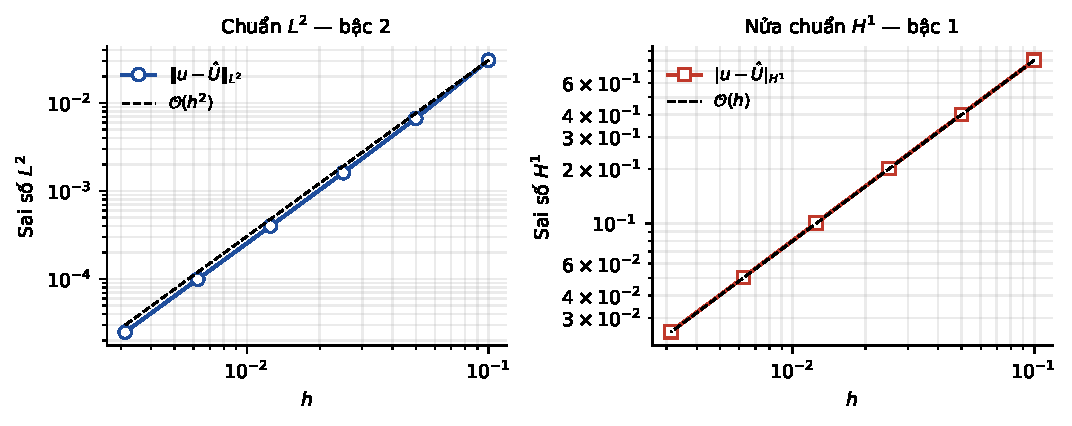
\includegraphics[width=\textwidth]{figures/fig_convergence.pdf}
\caption{Đồ thị log--log của sai số theo $h$ với $\theta = 0.5$. Đường đứt
nét là các đường tham chiếu $\mathcal{O}(h^{2})$ và $\mathcal{O}(h)$.}
\label{fig:convergence}
\end{figure}

Hình~\ref{fig:solution} so sánh nghiệm số với nghiệm chính xác. Tại
$t = 20$ (sau $20$ chu kỳ), biên độ nghiệm số \emph{không} tăng --- đúng như
Mệnh đề~\ref{prop:disc-energy} dự đoán --- sai số quan sát được chủ yếu là lệch
pha, tức tán sắc số.

\begin{figure}[H]
\centering
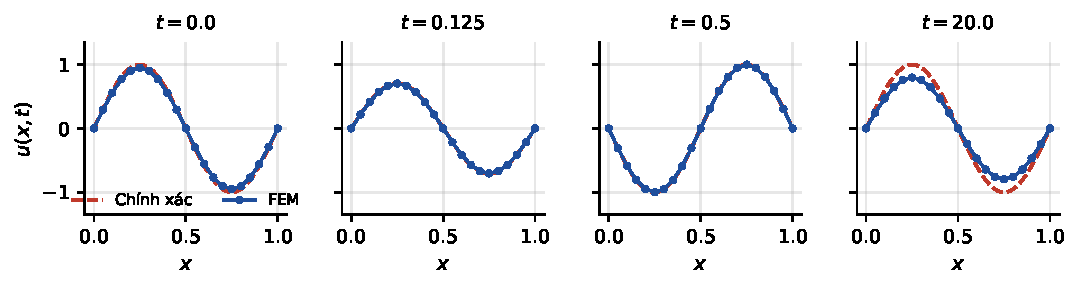
\includegraphics[width=\textwidth]{figures/fig_solution.pdf}
\caption{Nghiệm FEM ($N = 20$, $\theta = 0.5$) so với nghiệm chính xác.
Biên độ được bảo toàn sau $20$ chu kỳ; sai số dài hạn là sai số pha.}
\label{fig:solution}
\end{figure}

\subsection{Thực nghiệm 2: bậc hội tụ theo thời gian}

Để tách riêng sai số thời gian khỏi sai số không gian, ta cố định
$N = 200$ và so sánh các nghiệm ứng với $\dt$ giảm dần theo kiểu Richardson:
đại lượng $\norm{\hat U_{\dt} - \hat U_{\dt/2}}$ có cùng bậc với sai số
thời gian.

\begin{table}[H]
\centering
\caption{Bậc hội tụ theo thời gian, $N = 200$ cố định,
$T_{\mathrm{end}} = 1$.}
\label{tab:temporal}
\begin{tabular}{r r r c}
\toprule
$\theta = \dt/h$ & $\dt$
  & $\norm{\hat U_{\dt} - \hat U_{\dt/2}}_{\Ltwo}$ & bậc \\
\midrule
0.500000 & $2.500\times 10^{-3}$ & $1.023662\times 10^{-8}$ & ---  \\
0.250000 & $1.250\times 10^{-3}$ & $2.299690\times 10^{-9}$ & 2.15 \\
0.125000 & $6.250\times 10^{-4}$ & $5.586810\times 10^{-10}$ & 2.04 \\
0.062500 & $3.125\times 10^{-4}$ & $1.386980\times 10^{-10}$ & 2.01 \\
0.031250 & $1.563\times 10^{-4}$ & $3.466993\times 10^{-11}$ & 2.00 \\
\bottomrule
\end{tabular}
\end{table}

Bậc $2.00$ xác nhận Định lý~\ref{thm:temporal}, đồng thời khẳng định vai trò của
khởi tạo bậc hai \eqref{eq:init} như đã nêu ở Nhận xét~\ref{rem:init}.

\subsection{Thực nghiệm 3: định vị ngưỡng ổn định}

Đây là kiểm chứng trực tiếp cho Định lý~\ref{thm:spectrum}. Ta quét
$\theta = \dt/h$ và ghi lại $\max_{j}\lvert U_{j}^{M}\rvert$ sau
$M = \lfloor T_{\mathrm{end}}/\dt \rfloor$ bước, với dữ liệu ban đầu chuẩn
hóa $\max_{j}\lvert U_{j}^{0}\rvert = 1$. Để mode bất ổn định lộ ra ngay
(xem Nhận xét~\ref{rem:roundoff}), ta kích thích nó với biên độ $10^{-8}$.

\begin{table}[H]
\centering
\caption{Hệ số biên độ $\max_{j}\lvert U_{j}^{M}\rvert$ khi quét
$\theta$, khối lượng đầy đủ. Ngưỡng giải tích:
$\theta^{*}(N{=}80) = 0.577684$, $\theta^{*}(N{=}160) = 0.577434$;
giới hạn $h \to 0$ là $1/\sqrt{3} = 0.577350$.}
\label{tab:stability}
\begin{tabular}{r r r l}
\toprule
$\theta$ & $N = 80$ & $N = 160$ & Trạng thái \\
\midrule
0.5700 & $9.999\times 10^{-1}$ & $9.999\times 10^{-1}$ & ổn định \\
0.5774 & $9.997\times 10^{-1}$ & $1.000$               & ổn định \\
0.5776 & $9.998\times 10^{-1}$ & $1.002$               & $N{=}160$ vừa vượt ngưỡng \\
0.5778 & $9.998\times 10^{-1}$ & $2.362$               & $N{=}160$ phân kỳ \\
0.5780 & $9.999\times 10^{-1}$ & $2.065\times 10^{2}$  & $N{=}160$ phân kỳ \\
0.5800 & $2.242\times 10^{2}$  & $1.623\times 10^{14}$ & cả hai phân kỳ \\
\bottomrule
\end{tabular}
\end{table}

Ngưỡng thực nghiệm trùng khớp với $\theta^{*}$ giải tích tới \emph{bốn chữ
số có nghĩa}. Đáng chú ý, với $\theta = 0.5776$ thì $N = 160$ đã phân kỳ
trong khi $N = 80$ vẫn ổn định --- hoàn toàn nhất quán với
$\theta^{*}$ giảm dần theo $N$ như \eqref{eq:lambda-exact} tiên đoán.

Hình~\ref{fig:stability} cho thấy toàn cảnh: hai bậc thang dựng đứng xuất hiện
đúng tại $1/\sqrt{3}$ (khối lượng đầy đủ) và $1$ (khối lượng gộp), xác nhận
trọn vẹn \eqref{eq:cfl-two}.

\begin{figure}[H]
\centering
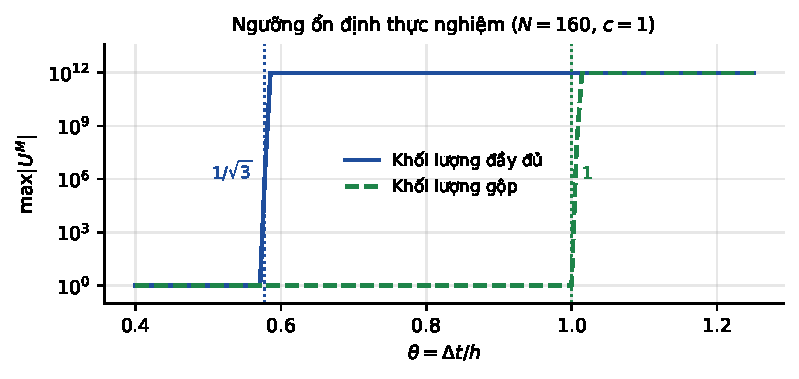
\includegraphics[width=0.82\textwidth]{figures/fig_stability.pdf}
\caption{Hệ số biên độ theo $\theta = \dt/h$ với $N = 160$. Ngưỡng ổn định
của khối lượng đầy đủ nằm tại $1/\sqrt{3} \approx 0.577$, của khối lượng gộp
tại $1$, đúng như Định lý~\ref{thm:spectrum}. Vượt ngưỡng, biên độ đạt tới
$10^{148}$ nên cả hai đường được chặn ở $10^{12}$ để vẽ; phần nằm ngang là
ngưỡng chặn hiển thị, không phải bình nguyên.}
\label{fig:stability}
\end{figure}

Hình~\ref{fig:energy} minh họa Mệnh đề~\ref{prop:disc-energy}: dưới ngưỡng, năng lượng
rời rạc là hằng số tới sai số máy suốt $20$ đơn vị thời gian; vượt ngưỡng
dù chỉ $0.4\%$, năng lượng bùng nổ theo cấp số nhân.

\begin{figure}[H]
\centering
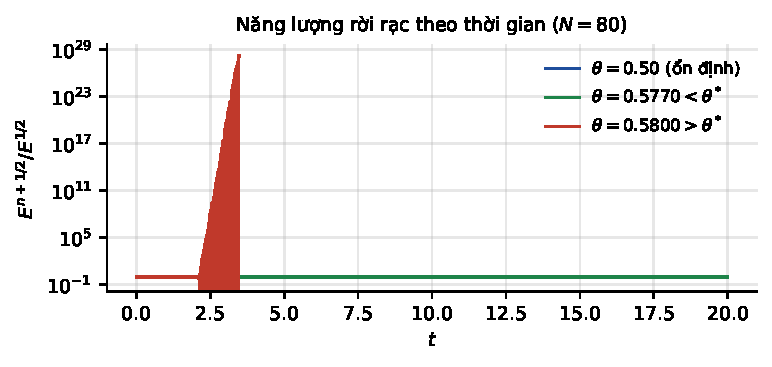
\includegraphics[width=0.72\textwidth]{figures/fig_energy.pdf}
\caption{Bao trên $\max_{m \leq n}$ của năng lượng rời rạc
$\mathcal{E}^{m+1/2}$ chuẩn hóa ($N = 80$). Với $\theta < \theta^{*}$ năng
lượng được bảo toàn tới sai số máy (hai đường ổn định lệch nhau $5\times
10^{-15}$, nên một đường vẽ nét đứt); với $\theta > \theta^{*}$ nó tăng theo
cấp số nhân. Vẽ bao trên thay vì tỉ số thô vì khi mất ổn định, mode trội đổi
dấu mỗi bước khiến $\mathcal{E}$ đi qua đúng $0$ --- điều mà trục log không
biểu diễn được.}
\label{fig:energy}
\end{figure}

\subsection{Thực nghiệm 4: hiệu quả của khối lượng gộp}

Cuối cùng, ta lặp lại Thực nghiệm 1 với ma trận khối lượng gộp và
$\theta = 0.9$ --- giá trị \emph{vượt} ngưỡng của khối lượng đầy đủ nhưng
vẫn nằm trong ngưỡng $\theta < 1$ của khối lượng gộp.

\begin{table}[H]
\centering
\caption{Sai số và bậc hội tụ với ma trận khối lượng gộp, $\theta = 0.9$.
Bước thời gian lớn hơn $56\%$ so với Bảng~\ref{tab:conv} mà vẫn ổn định.}
\label{tab:lumped}
\begin{tabular}{r r r c r c}
\toprule
$N$ & $h$
 & $\norm{u-\hat U}_{\Ltwo}$ & bậc
 & $\seminorm{u-\hat U}_{\Hone}$ & bậc \\
\midrule
 10 & 0.100000 & $2.5370\times 10^{-2}$ & ---  & $8.0057\times 10^{-1}$ & ---  \\
 20 & 0.050000 & $6.3636\times 10^{-3}$ & 2.00 & $4.0226\times 10^{-1}$ & 0.99 \\
 40 & 0.025000 & $1.5922\times 10^{-3}$ & 2.00 & $2.0138\times 10^{-1}$ & 1.00 \\
 80 & 0.012500 & $3.9815\times 10^{-4}$ & 2.00 & $1.0072\times 10^{-1}$ & 1.00 \\
160 & 0.006250 & $9.9542\times 10^{-5}$ & 2.00 & $5.0364\times 10^{-2}$ & 1.00 \\
320 & 0.003125 & $2.4886\times 10^{-5}$ & 2.00 & $2.5183\times 10^{-2}$ & 1.00 \\
\bottomrule
\end{tabular}
\end{table}

Khối lượng gộp giữ nguyên bậc hội tụ $\mathcal{O}(h^{2})$, thậm chí sai số
$\Ltwo$ còn \emph{nhỏ hơn} chút ít, đồng thời cho phép bước thời gian lớn
hơn $\sqrt{3} \approx 1.73$ lần và biến việc giải hệ thành phép chia vô
hướng. Đây là lựa chọn ưu việt rõ rệt cho bài toán sóng.

%=======================================================================
\section{Kết luận}
\label{sec:ketluan}

Báo cáo đã xây dựng, phân tích và kiểm chứng đầy đủ phương pháp phần tử hữu
hạn $P_{1}$ kết hợp sai phân trung tâm cho phương trình sóng một chiều. Các
kết luận chính:

\begin{enumerate}
  \item \textbf{Về lý thuyết.} Phương pháp hội tụ với bậc
        $\mathcal{O}(h^{2} + \dt^{2})$ trong chuẩn $\Ltwo$ và
        $\mathcal{O}(h + \dt^{2})$ trong nửa chuẩn $\Hone$
        (Định lý~\ref{thm:total}). Việc dùng phép chiếu Ritz thay cho phép nội suy
        làm chứng minh gọn hơn hẳn và loại bỏ nhu cầu dùng bổ đề
        Aubin--Nitsche.
  \item \textbf{Về ổn định.} Điều kiện cần và đủ là
        $\dt < 2/(c\sqrt{\lammax})$ (Định lý~\ref{thm:cfl}). Tính tường minh phổ
        cho hai hằng số CFL khác biệt: $h/(c\sqrt{3})$ cho khối lượng đầy đủ
        và $h/c$ cho khối lượng gộp (Định lý~\ref{thm:spectrum}). Vì vậy
        \emph{ước lượng quen thuộc $\dt \le h/c$ là không đủ} khi dùng khối
        lượng đầy đủ --- một cái bẫy dễ mắc trong thực hành.
  \item \textbf{Về thực nghiệm.} Bậc hội tụ đo được trùng khớp lý thuyết
        ($2.00$ và $1.00$), và ngưỡng ổn định thực nghiệm trùng với dự đoán
        giải tích tới bốn chữ số có nghĩa.
  \item \textbf{Về thực hành.} Khối lượng gộp là lựa chọn được khuyến nghị:
        giữ nguyên bậc chính xác, cho phép $\dt$ lớn hơn $\sqrt{3}$ lần, và
        loại bỏ hoàn toàn chi phí giải hệ tuyến tính mỗi bước.
\end{enumerate}

\subsection*{Hướng phát triển}

\begin{itemize}
  \item Mở rộng lên hai và ba chiều, nơi điều kiện CFL trở thành
        $\dt \le h/(c\sqrt{d})$ với $d$ là số chiều, và khối lượng gộp càng
        có lợi do chi phí giải hệ tăng nhanh.
  \item Dùng phần tử bậc cao $p \ge 2$ để đạt bậc hội tụ cao hơn; khi đó cần
        tính lại $\lammax$ vì hằng số CFL phụ thuộc $p$ (giảm dần theo
        $p^{2}$).
  \item Khảo sát các sơ đồ thời gian ẩn (Newmark, trung điểm) vốn ổn định vô
        điều kiện, đánh đổi bằng chi phí giải hệ ở mỗi bước.
  \item Phân tích sai số tán sắc (phase error) một cách định lượng, vì như
        Hình~\ref{fig:solution} cho thấy đây mới là nguồn sai số trội trong mô
        phỏng dài hạn.
\end{itemize}

%=======================================================================
\begin{thebibliography}{9}
\bibitem{brenner2008}
S.~C. Brenner and L.~R. Scott,
\emph{The Mathematical Theory of Finite Element Methods},
3rd ed., Springer, New York, 2008.

\bibitem{ciarlet2002}
P.~G. Ciarlet,
\emph{The Finite Element Method for Elliptic Problems},
SIAM Classics in Applied Mathematics, Philadelphia, 2002.

\bibitem{thomee2006}
V.~Thomée,
\emph{Galerkin Finite Element Methods for Parabolic Problems},
2nd ed., Springer, Berlin, 2006.

\bibitem{cohen2002}
G.~C. Cohen,
\emph{Higher-Order Numerical Methods for Transient Wave Equations},
Springer, Berlin, 2002.

\bibitem{hughes2000}
T.~J.~R. Hughes,
\emph{The Finite Element Method: Linear Static and Dynamic Finite Element
Analysis}, Dover, New York, 2000.

\bibitem{leveque2007}
R.~J. LeVeque,
\emph{Finite Difference Methods for Ordinary and Partial Differential
Equations}, SIAM, Philadelphia, 2007.

\bibitem{strang2008}
G.~Strang and G.~J. Fix,
\emph{An Analysis of the Finite Element Method},
2nd ed., Wellesley-Cambridge Press, 2008.
\end{thebibliography}

%=======================================================================
\appendix
\section{Mã nguồn tái lập kết quả}
\label{app:code}

Toàn bộ kết quả số trong Mục~\ref{sec:thucnghiem} được sinh bởi đoạn mã dưới
đây (Python 3 với \texttt{NumPy}). Hàm \texttt{solve} trả về cặp sai số
$(\norm{\cdot}_{\Ltwo}, \seminorm{\cdot}_{\Hone})$ tại thời điểm cuối; hàm
\texttt{lam\_max} tính $\lammax$ theo công thức giải tích
\eqref{eq:lambda-exact}.

\lstinputlisting[style=py, caption={Cài đặt FEM $P_1$ + leapfrog cho phương
trình sóng một chiều.}, label={lst:code}]{fem_wave.py}

\end{document}
